%CLASSE DOCUMENTO - LINGUA E DIMENSIONE FONT
\documentclass[trieste,corpo=11pt,numerazioneromana]{toptesi}

%%%%%%%%%%%%%%%%%%%%%%%%%%%%%%%%%%%%%%%%%%%%%%%%%%%%%%%%%%%%%%%

% INCLUSIONE PACCHETTI
\usepackage[classica]{topfront}
\usepackage[utf8]{inputenc} %utf8
\usepackage[italian]{babel}
\usepackage[T1]{fontenc}
\usepackage{blindtext}
\usepackage{graphicx,wrapfig}
\usepackage{booktabs}
\usepackage{lmodern}
\usepackage{varioref}
\usepackage{epigraph}
\usepackage{url}
\usepackage{array}
\usepackage{paralist}{\obeyspaces\global\let =\space}
\usepackage{verbatim}
\usepackage{subfig}
\usepackage{tabularx}
\usepackage{amsmath}
\usepackage{amsfonts}
\usepackage{float}
\usepackage{float}
\usepackage{amssymb}
\usepackage{multicol}
\usepackage{multirow}
\usepackage{listings}
\usepackage[pass]{geometry}
\usepackage[figuresright]{rotating}
\usepackage{algorithm}
\usepackage{algorithmic}
\usepackage{wrapfig}
\usepackage{amsmath}
\usepackage[babel]{csquotes}
\usepackage{hyperref}
\usepackage[backend=biber,bibencoding=ascii]{biblatex}


%%%%%%%%%%%%%%%%%%%%%%%%%%%%%%%%%%%%%%%%%%%%%%%%%%%%%%%%%%%%%%%

% CONFIGURAZIONE LINK E RIFERIMENTI
\hypersetup{%
    pdfpagemode={UseOutlines},
    bookmarksopen,
    pdfstartview={FitH},
    colorlinks,
    linkcolor={black}, %COLORE DEI RIFERIMENTI AL TESTO
    citecolor={blue}, %COLORE DEI RIFERIMENTI ALLE CITAZIONI
    urlcolor={blue} %COLORI DEGLI URL
}

%%%%%%%%%%%%%%%%%%%%%%%%%%%%%%%%%%%%%%%%%%%%%%%%%%%%%%%%%%%%%%%

% CONFIGURAZIONE LISTATI/CODICE - CANCELLARE SE NON NECESSARIO
% PYTHON - BIANCO E NERO
\lstset{%
	captionpos=b,
	language=Python,
	basicstyle =\small\ttfamily,
	keywordstyle=\color{black}\bfseries,
	breaklines=true,
	breakatwhitespace=true,
	frame=lines,
	numbers=left,
	numberstyle=\footnotesize,
}

%%%%%%%%%%%%%%%%%%%%%%%%%%%%%%%%%%%%%%%%%%%%%%%%%%%%%%%%%%%%%%%

% FRENCHSPACING VA _SEMPRE_ ABILITATO PER DOCUMENTI IN ITALIANO
\frenchspacing

%%%%%%%%%%%%%%%%%%%%%%%%%%%%%%%%%%%%%%%%%%%%%%%%%%%%%%%%%%%%%%%

%DEFINIZIONE SEZIONI IN NUMERAZIONE ROMANA
%ELENCO DEI LISTATI/CODICI
\makeatletter
\newcommand\listofcodes{%
 \iffrontmatter\else\frontmattertrue\fi
 \if@openright\cleardoublepage\else\clearpage\fi
 % change the meaning of \chapter in a group
 \begingroup\def\chapter##1{\@schapter}
 \phantomsection % for the hyperlink
 \addcontentsline{toc}{chapter}{Elenco dei listati}
 \lstlistoflistings
 \endgroup
}
\makeatother

\addto\captionsitalian{%
  \renewcommand{\lstlistlistingname}{Elenco dei listati}%
  \renewcommand{\lstlistingname}{Listato}%
}

%%%%%%%%%%%%%%%%%%%%%%%%%%%%%%%%%%%%%%%%%%%%%%%%%%%%%%%%%%%%%%%

% INFORMAZIONI PDF - PERSONALIZZARE
\pdfinfo{%
  /Title    (Realizzazione di un assistente vocale per il triage ospedaliero)
  /Author   (Simone Montali)
  /Subject  (Triage semi-automatizzato per la sicurezza e la tempestività)
  /Keywords (Triage ML Mycroft Ospedale Hospital)
}

%%%%%%%%%%%%%%%%%%%%%%%%%%%%%%%%%%%%%%%%%%%%%%%%%%%%%%%%%%%%%%%

% LISTA DEI CAPITOLI DA INCLUDERE - PERSONALIZZARE
\includeonly{%
introduzione,%
stateofart,%
mycroft,%
app_a,%
}

% FILE DI BIBLIOGRAFIA
\addbibresource{bibliography.bib}

%%%%%%%%%%%%%%%%%%%%%%%%%%%%%%%%%%%%%%%%%%%%%%%%%%%%%%%%%%%%%%%

% INIZIO DOCUMENTO
\begin{document}

%%%%%%%%%%%%%%%%%%%%%%%%%%%%%%%%%%%%%%%%%%%%%%%%%%%%%%%%%%%%%%%

% FRONTESPIZIO - PERSONALIZZARE
% ELIMINATE LE VOCI CHE NON VI SERVONO

% UNIVERSITA - NOME
\ateneo{Università degli studi di Parma}

% FACOLTA - DICITURA - CANCELLARE O DECOMMENTARE
%\FacoltaDi{Faculty of}
% FACOLTA - NOME
\facolta{Ingegneria}

% CORSO DI LAUREA - DICITURA (MANTENERE LO SPAZIO) - CANCELLARE O DECOMMENTARE
%\CorsoDiLaureaIn{Master of Science in }
% CORSO DI LAUREA - NOME
\corsodilaurea{Ingegneria dei Sistemi Informativi}

% TIPOLOGIA TESI
\TesiDiLaurea{Tesi di Laurea di primo livello}

% TITOLO
\titolo{Realizzazione di un assistente vocale per il triage ospedaliero}

% SOTTOTITOLO
\sottotitolo{Triage semi-automatizzato per la sicurezza e la tempestività}

% RELATORE/I - DICITURA - CANCELLARE SE UN SOLO RELATORE
\AdvisorName{Relatori}
% RELATORE - PROF. NOME E COGNOME
\relatore{prof.ssa\ Mordonini Monica}
% RELATORE AGGIUNTIVO - PROF NOME E COGNOME
% SE SI HA SOLO UN RELATORE ELIMINARE INSIEME AD AdvisorName
\terzorelatore{prof.\ Tomaiuolo Michele}
%\terzorelatore{prof.\ Angiani Giulio}
% CANDIDATO - DICITURA (MANTENERE I DUE PUNTI) - CANCELLARE O DECOMMENTARE
%\CandidateName{Candidate:}

% CANDIDATO - NOME E COGNOME
\candidato{Simone Montali}[288144]

% LOGO UNIVERSITA
\logosede{images/logo}

% DATA - MESE ANNO
\sedutadilaurea{Probabilmente 2020}

\frontespizio

%%%%%%%%%%%%%%%%%%%%%%%%%%%%%%%%%%%%%%%%%%%%%%%%%%%%%%%%%%%%%%%

%INTERLINEA - DEFAULT 1 - NON ESAGERATE, NON SUPERATE MAI 1.3 ;)
%\interlinea{1.2}

%%%%%%%%%%%%%%%%%%%%%%%%%%%%%%%%%%%%%%%%%%%%%%%%%%%%%%%%%%%%%%%

\frontmatter

% DEDICA - PERSONALIZZARE
% VSPACE - PROPORZIONE USATA PER CENTRATURA VERTICALE DEL TESTO
% FLUSHRIGHT - ALLINEAMENTO ORIZZONTALE A DESTRA
\vspace*{\stretch{1}}
\begin{flushright}
  \noindent
  Dedica toccante.
\end{flushright}
\vspace*{\stretch{6}}
\cleardoublepage


% CITAZIONE - PERSONALIZZARE
% VSPACE - PROPORZIONE USATA PER CENTRATURA VERTICALE DEL TESTO
% FLUSHRIGHT - ALLINEAMENTO ORIZZONTALE A DESTRA
\vspace*{\stretch{1}}
\begin{flushright}
  \noindent
  Citatemi dicendo che sono stato citato male.

  \textit{Groucho Marx}
\end{flushright}
\vspace*{\stretch{6}}
\cleardoublepage

%%%%%%%%%%%%%%%%%%%%%%%%%%%%%%%%%%%%%%%%%%%%%%%%%%%%%%%%%%%%%%%

% RINGRAZIAMENTI - PERSONALIZZARE
\ringraziamenti
Grazie

%%%%%%%%%%%%%%%%%%%%%%%%%%%%%%%%%%%%%%%%%%%%%%%%%%%%%%%%%%%%%%%

% ABSTRACT - PERSONALIZZARE
\sommario
Abstract della tesi
%%%%%%%%%%%%%%%%%%%%%%%%%%%%%%%%%%%%%%%%%%%%%%%%%%%%%%%%%%%%%%%

% INDICI - ELIMINARE GLI INDICI NON NECESSARI

% INDICE GENERALE
\tableofcontents

% INDICE DELLE FIGURE
\listoffigures

% INDICE DELLE TABELLE
%\listoftables

% INDICE DEI CODICI
%\listofcodes

%%%%%%%%%%%%%%%%%%%%%%%%%%%%%%%%%%%%%%%%%%%%%%%%%%%%%%%%%%%%%%%

\mainmatter

% INCLUSIONE FILE CAPITOLI - PERSONALIZZARE - TENERE COERENTE CON LISTA IN ALTO
\chapter{Introduzione}
\label{chap:introduzione}
In una società sempre più digitalizzata e dinamica, spesso viene a crearsi un netto distacco tra i settori capaci di \textbf{evolvere assieme alla tecnologia}, e quelli che, per un motivo o per l'altro, rimangono ancorati a procedure e metodologie tradizionali. Il settore medico, in continuo rinnovamento sul lato scientifico, è, soprattutto in Italia, affidato ad \textbf{infrastrutture informatiche progettate tempo fa.} Questo, soprattutto per motivi di stabilità e affidabilità: gli errori, qui, non sono ammissibili. \\
Per questo motivo, spesso non si notano le evidenti possibilità di miglioramenti che la ricerca informatica potrebbe apportare agli ospedali, agli ambulatori, agli studi.
L'obiettivo di questa tesi è mettere luce su una delle possibili modalità con cui l'informatica potrebbe, in un futuro prossimo, migliorare la praticità ma soprattutto la sicurezza degli ambienti ospedalieri.\\
La procedura di triage, ossia il processo di selezione dei pazienti richiedenti cure, è oggi affidata totalmente ad infermieri. Questa scelta è dovuta, oltre ad un evidente bisogno di poter osservare il paziente, alla necessità dell'\textbf{immediatezza di un contatto verbale} con il personale sanitario. \\
Perciò, la sfida nella realizzazione della tesi è soprattutto legata al rendere il \textbf{più umana possibile} l'interazione con un bot automatizzato. Il bot deve quindi accogliere il paziente, comprenderne le problematiche ed i sintomi, e farlo sentire protetto. Non si escluderà del tutto un apporto umano: gli infermieri sono addestrati per poter osservare e comprendere il richiedente cura, e l'apporto dell'osservazione diretta del paziente è ancora troppo importante per escluderla. È senz'altro possibile, però, affidare la prima parte di \textbf{profilazione dell'utente} a procedure automatizzate.

\chapter{Stato dell'arte}
\label{chap:stateofart}
Impara l'arte e mettila da parte.

\chapter{Mycroft}
\label{chap:mycroft}
\epigraph{There’s an entire community of developers looking to access this technology, but so far, it’s been the purview of a few large companies. The technology is walled-off, proprietary, and secretive.}{\textit{Joshua Montgomery \\ CEO di Mycroft AI, Inc.}}
Nel panorama degli assistenti vocali disponibili al pubblico, le grandi aziende catturano la maggior parte delle attenzioni dei consumatori. I nomi di Amazon Alexa, Google Home, Microsoft Cortana sono familiari a tanti. Meno familiare, però, è lo scenario degli stessi strumenti in ambito di assistenti vocali. Piattaforme come \textit{Jarvis}, \textit{Linto}, \textit{Open Assistant} e \textbf{Mycroft} sono sconosciute ai più. Quest'ultimo, negli ultimi anni, ha catturato l'attenzione di molti esperti di settore per la sua stabilità, espansibilità, popolarità.
\section{Open source}
\subsection{Cosa si intende con open source?}
Il termine \textbf{open source} si riferisce a qualcosa di modificabile e condivisibile dalle persone, avente quindi un \textbf{design pubblicamente accessibile.} Il termine nacque nell'ambito dello sviluppo software, ma oggi rappresenta, piuttosto, un'etica. Il software open source è software il cui codice sorgente è ispezionabile, modificabile, e migliorabile da chiunque voglia farlo. Con \textit{codice sorgente} intendiamo il codice che definisce il comportamento del programma, ossia il prodotto del lavoro di un programmatore. \\
Molti dei software che oggi utilizziamo sono invece \textbf{closed source} (o \textit{proprietario}), ossia software il cui codice sorgente non è accessibile agli utenti, e sul quale l'organizzazione che crea il software ha \textit{pieni poteri}. Alcuni esempi di software proprietario possono essere Windows, Photoshop, Safari. Solitamente, durante l'installazione di uno di questi software, l'utente accetta dei termini e condizioni che lo vincolano a non fare nulla di non autorizzato dall'azienda creatrice del software.
\subsection{Perché open source?}
Le motivazioni per preferire software open source rispetto a quelli proprietari sono svariate. Sebbene i software proprietari spesso abbiano funzionalità più avanzate e, spesso, meglio sviluppate, hanno gravi mancanze in progetti come questo. Il software open source, a scapito della possibilità di minori funzionalità (nonostante ciò non sia sempre vero, basti pensare alla potenza del kernel Linux), dà ad un utente esperto tante possibilità:
\begin{itemize}
    \item Possibilità di \textbf{controllo} sul software: la modifica e il miglioramento del software è permessa e ben vista. La comunità open source lavora con coesione per produrre software sempre migliore.
    \item Possibilità di conoscere e studiare i \textbf{meccanismi interni}: l'utilizzo di software per fini scientifici richiede la piena conoscenza di come un software funziona. Inoltre, la disponibilità del codice a tutti permette agli studenti e agli interessati di scoprire le logiche che ne permettono il corretto funzionamento.
    \item Grandi garanzie di \textbf{sicurezza}: se tutti possono accedere al codice, la presenza di bug di sicurezza e problematiche di privacy viene rilevata molto più velocemente di come accade nel software proprietario.
    \item Certezze sulla \textbf{privacy}: la società in cui viviamo è sempre più basata sulla vendita di dati personali acquisiti tramite software. L'open source, spesso e volentieri, si oppone a tale tendenza: essendo software della comunità e non di un'azienda che punta all'ottenimento di capitale, nessuno ha interesse nel \textit{monetizzare gli utenti}.
    \item Supporto della \textbf{comunità}: lo sviluppo di software open source è molto supportato dalla comunità informatica. In caso di problematiche o necessità, ci sarà sempre un utente più esperto disposto ad aiutare.
    \item Correttezza \textbf{etica}: software come quello oggetto di questa tesi hanno l'obiettivo di salvare vite. È giusto che tutti possano accedervi, migliorarlo e conoscerlo. La ricerca scientifica dovrebbe essere il più possibile \textbf{libera}.
\end{itemize}
\section{Introduzione a Mycroft}
Mycroft nacque tramite crowdfunding nel 2015 e catturò subito molto interesse da parte della comunità informatica. L'obiettivo era chiaro: opporsi alla sola presenza di software proprietario nel campo degli assistenti vocali. Ricevette presto l'appoggio di molte organizzazioni come la Canonical (promotrice di Ubuntu) e la Mozilla Foundation. La repository su Github di Mycroft conta oggi \textit{4300 stars} in continua crescita.
\subsection{Stack di funzionamento}
Come spiegato nel capitolo \ref{section:vocal_assistants}, un assistente vocale si compone principalmente di:
\subsubsection{Rilevamento della wake word}
L'assistente ha bisogno di rilevare una parola per attivarsi. Gli esempi più famosi sono \textit{Hey, Google} o \textit{Alexa}. Mycroft permette di personalizzare la propria wake word, che all'installazione è semplicemente \textit{Hey, Mycroft}. Il progetto utilizza \textbf{Precise}, un wake word listener basato su reti neurali addestrate su esempi audio. Questo componente, totalmente open source, è basato su \textit{pattern sonori}, non sul testo. La caratteristica ne riduce la dipendenza da accenti e linguaggi diversi. Precise offre la possibilità di addestrare il listener su un proprio dataset. Il funzionamento è basato su una singola rete neurale ricorrente, più precisamente una \textbf{Gated Recurrent Unit} o GRU.
\begin{figure}[H]
    \begin{center}
        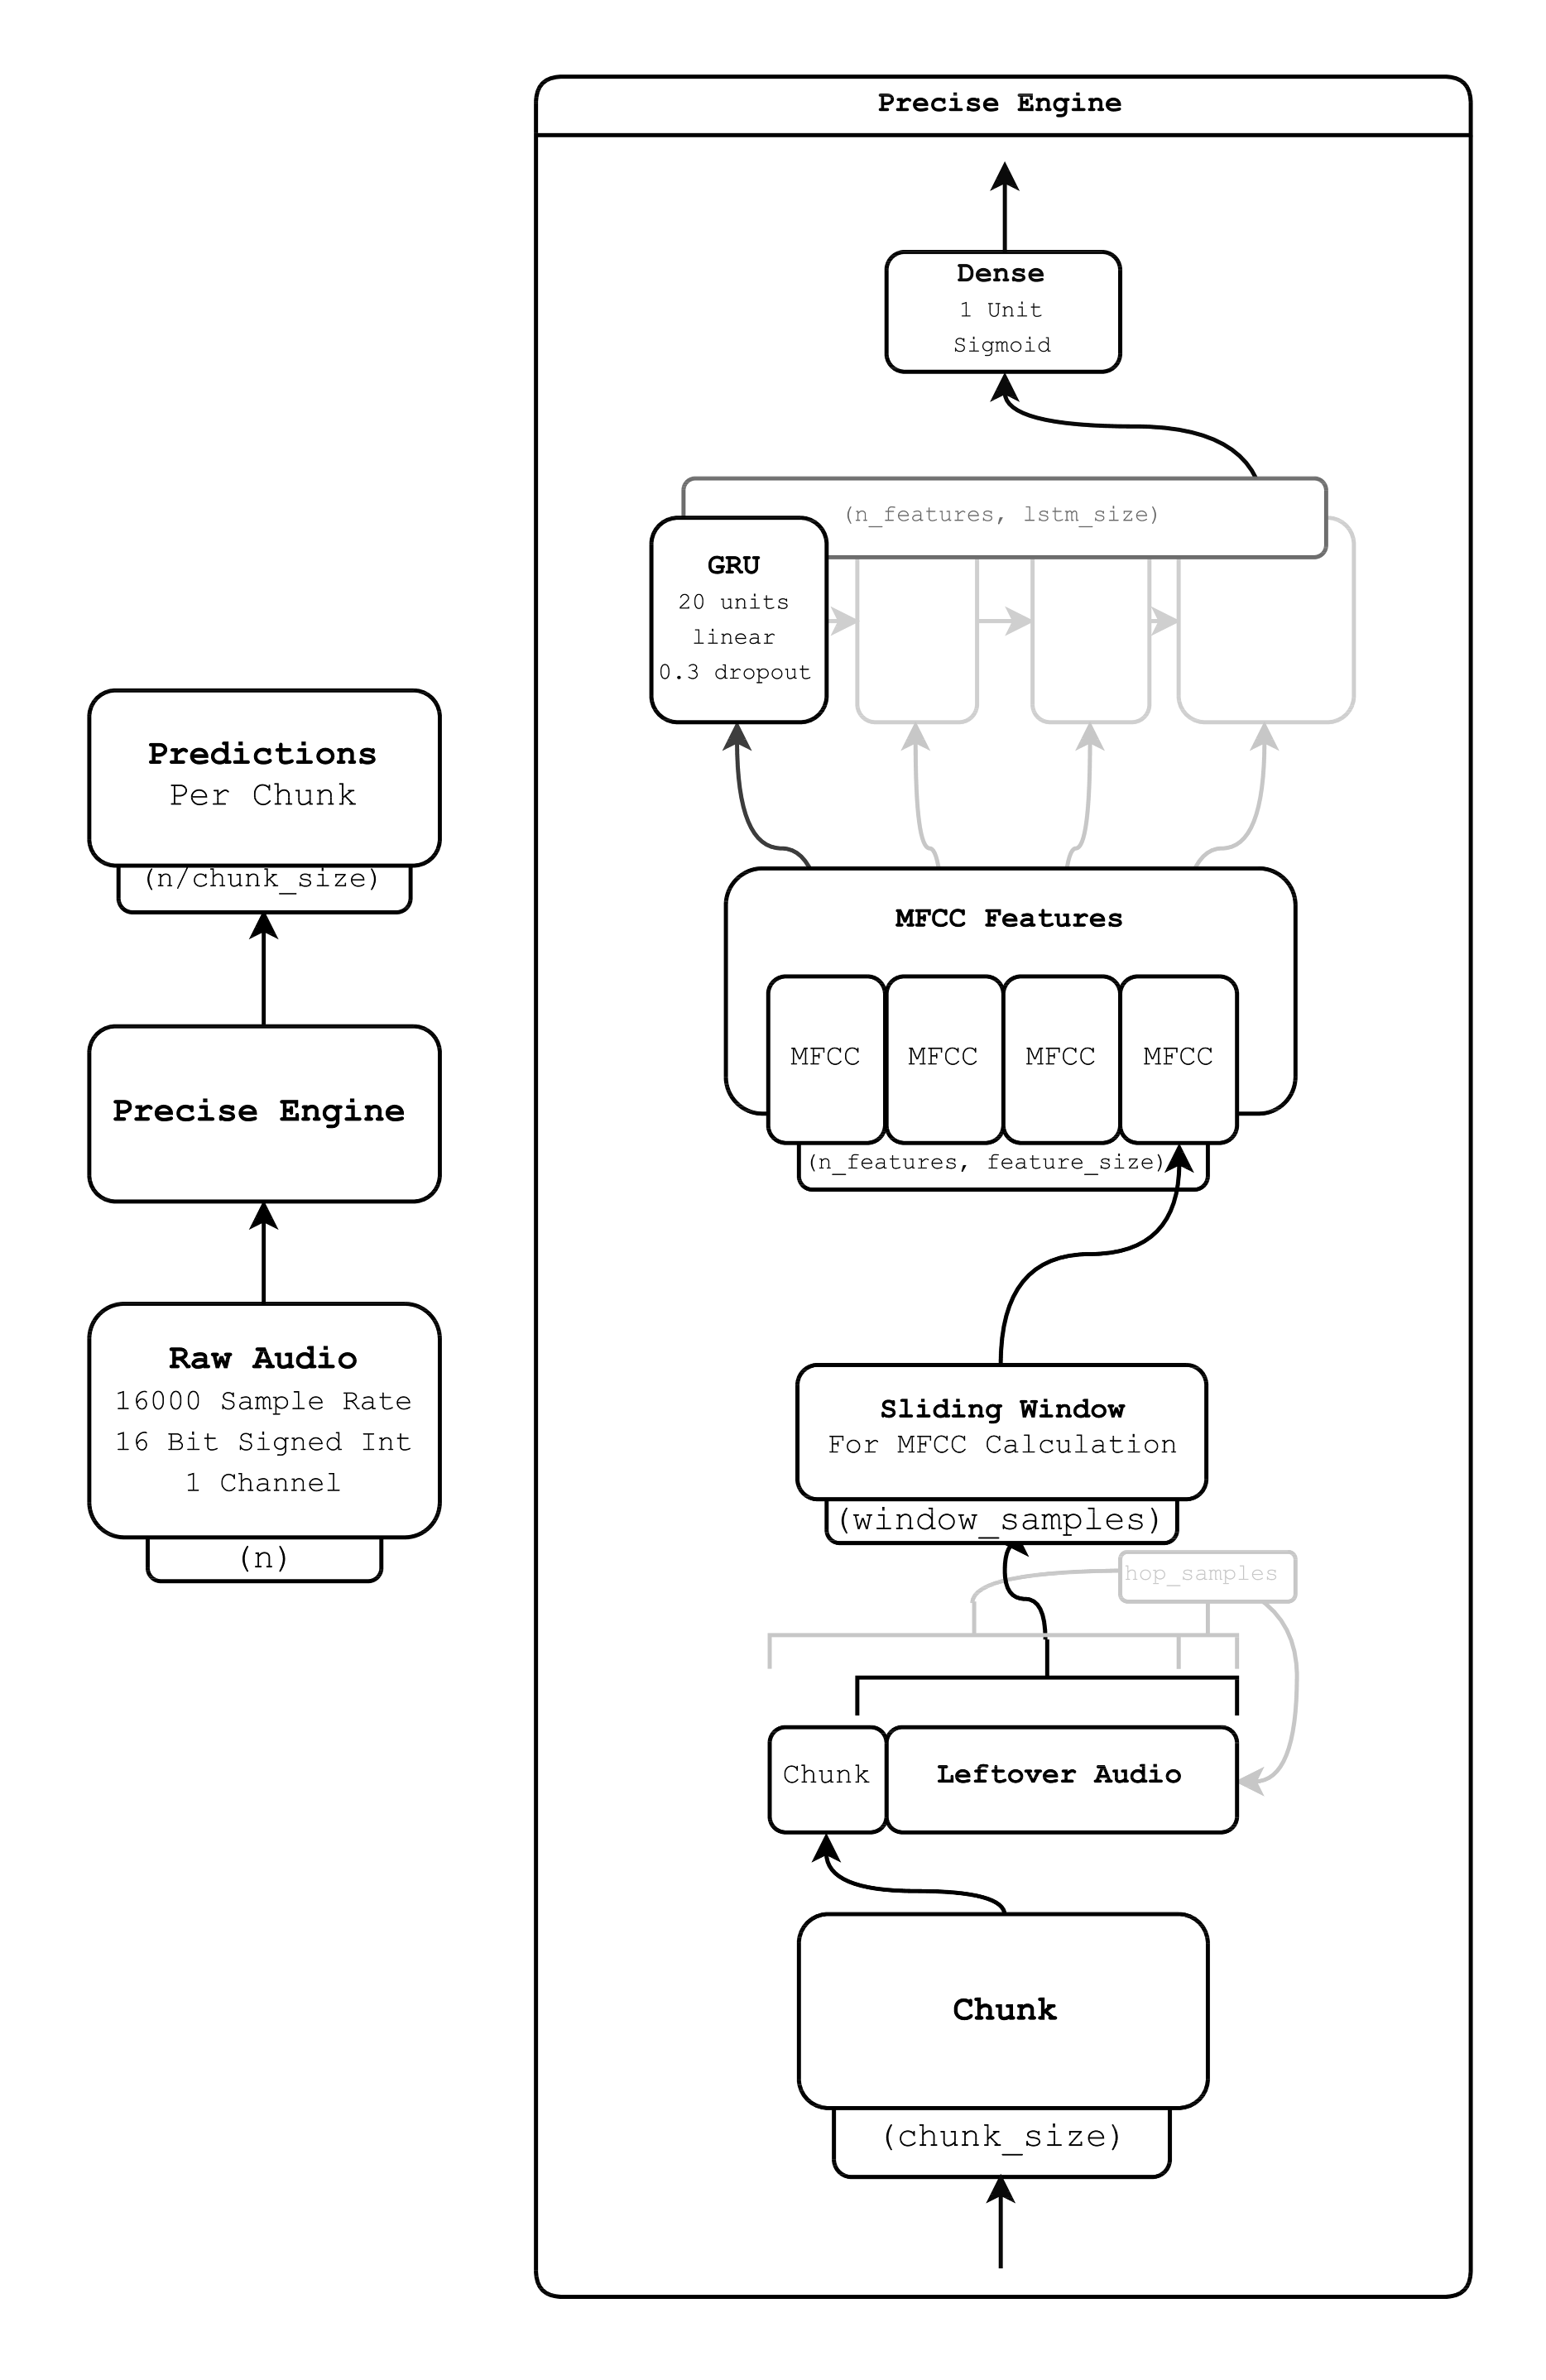
\includegraphics[width=0.6\columnwidth]{images/mycroft/precise.png}
    \end{center}
    \caption{Schema di funzionamento di Precise}
    \label{fig:precise}
\end{figure}
\subsubsection{Speech To Text}
Mycroft sfrutta il motore STT di Google per effettuare questo processo. Per aggiungere uno strato di privacy a queste richieste, esse vengono fatte passare attraverso i server Mycroft: Google non può ricollegare una richiesta all'utente che l'ha fatta. In questo modo, tutte le query effettuate a Google contengono solamente l'audio e hanno lo stesso mittente. In futuro sarà possibile sfruttare il dataset di \textbf{Mozilla Deepspeech}, che non è, ad oggi, ancora sufficientemente affidabile.
\subsubsection{Interpretazione degli intent}
Nell'ambito della speech recognition, un intent è l'operazione che l'utente \textit{intende} svolgere. Un utente può richiedere un'operazione in modi molto diversi. Lo scopo dell'intent parser è proprio quello di riuscire a superare questo scoglio, estraendo dalla richiesta scritta gli elementi chiave. Per esempio, se avessimo una richiesta del tipo "Hey Mycroft, domani pioverà a Parma?", l'intent parser dovrebbe capire:
\begin{itemize}
    \item L'utente desidera conoscere il \textbf{tempo atmosferico}.
    \item Il tempo atmosferico deve essere cercato per \textbf{Parma}.
    \item La data di interesse è \textbf{domani}.
\end{itemize}
Mycroft rende disponibili due software per la rilevazione di intenti: Padatious e Adapt. Mentre il secondo è basato sul riconoscimento di parole chiave, ed è quindi molto suscettibile alle richieste, il primo è composto da una rete neurale addestrata su frasi intere. Nel corso del progetto sfrutteremo \textbf{Padatious}.
Questo motore permette di avere creazione semplice degli intent, quantità di dati relativamente bassa, estrazione delle \textit{entities} semplice, addestramento rapido.
\subsubsection{Text To Speech}
Il componente di Text To Speech ha il compito di generare una traccia audio partendo dal testo di risposta codificato nella skill. Mycroft rende disponibile il progetto \textbf{Mimic}, basato sul software FLITE dell'università Carnegie Mellon. Purtroppo quest'ultimo non è disponibile in italiano, quindi nel corso del progetto utilizzeremo il motore TTS di Google, ottimizzato per l'italiano. Come sempre, le richieste passano attraverso i server Mycroft per ottenere un buon livello di privacy.
I testi di risposta sono codificati nei file vocabolario delle skills.
\subsection{Interfaccia grafica}
I dispositivi più avanzati di Mycroft come il \textit{Mark II} forniscono la possibilità di aggiungere interazioni visive con gli utenti. L'interfaccia è gestita da Mycroft-GUI, un componente aggiuntivo del bot che sfrutta i KDE Plasmoids, oggetti dell'interfaccia grafica KDE Plasma, simili a widget. La tecnologia è basata sul linguaggio QML, che permette una totale libertà nella creazione di interfacce, ma anche dei template standard semplici e rapidi da implementare. QML fa parte dello stack di tecnologie di Qt, una libreria multipiattaforma per lo sviluppo di programmi con interfaccia grafica.

\appendix
% INCLUSIONE APPENDICI - - PERSONALIZZARE - TENERE COERENTE CON LISTA IN ALTO
\chapter{An appendix}
\label{app:a}
% DA RIMUOVERE - LOREM IPSUM PER DIMOSTRAZIONE
\foreignlanguage{english}{\Blindtext}


%%%%%%%%%%%%%%%%%%%%%%%%%%%%%%%%%%%%%%%%%%%%%%%%%%%%%%%%%%%%%%%

% BIBLIOGRAFIA
\phantomsection
\addcontentsline{toc}{chapter}{\refname}
\nocite{*}
\printbibliography

\end{document}
